\chapter{Background}\label{ch:background}



\section{Uncertainty Quantification in Deep Learning}\label{back_uqdl}
In the last decade or so, deep learning has revolutionized learning-based methods, achieving great success in many fields, especially domains containing unstructured data such as computer vision, 3D modelling, and natural language processing. Deep learning models (e.g., neural networks) are usually deterministic in nature, learning machine-comprehensible representations that map high-dimensional input features to an array of outputs as predictions~\cite{ReprLearn}. Such models generally show high overall accuracy and are often accepted as correct without question. Unfortunately, that is not always the case, and such models quite frequently make over-confident predictions that are unexpected or not accurate, particularly in more complex real-world settings~\cite{DLDifficult1, DLDifficult2}, which can have serious consequences if not handled precisely~\cite{DLDisaster1, DLDisaster2, DLDisaster3, DLDisaster4}. Therefore, it is critical to recognize what is not precisely known to any deep learning model before using the model's prediction. To understand it quantitatively, appropriate numerical values must be assigned regarding the unknown variability of the prediction, known as uncertainty quantification (UQ). In deep learning modelling, there are two main kinds of uncertainty involved, namely aleatoric or data uncertainty and epistemic or model uncertainty~\cite{UncertDeepL}.
\newline

Aleatoric uncertainty refers to the inherent uncertainty in the data, which originates from the randomness or stochasticity of the data measurement, sampling, or the data generation process. For example, sensor or motion noise, and class confusion in training labels can contribute to data uncertainty~\cite{UncertDeepL}. This uncertainty cannot be reduced even with more training data and can be modelled by assuming a distribution over the model's predictions (e.g., Gaussian noise over regression model outputs). Data uncertainty can be homoscedastic (independent of inputs) or heteroscedastic (changes based on the input). In vision-related applications, modelling heteroscedastic data uncertainty is particularly important~\cite{UncertDeepL}.
\\
Epistemic uncertainty accounts for the uncertainty in prediction due to the model's variability in the training or inference process or uncertainty in learning the model parameters, and explains our lack of knowledge about the data-generating model. It comes from the limited availability of training data, model architecture (different initializations or hyperparameters), and out-of-distribution (OOD) test data. Unlike data uncertainty, this uncertainty can be reduced with more training data. It is modeled by assuming a prior distribution (e.g. Gaussian prior) over the weights of the model and computing the posterior distribution of the weights given some data. Such a setting is usual in Bayesian deep learning~\cite{UncertDeepL2, BayesNN}. 
\newline

Numerous works related to UQ in deep learning models have been done. While some approaches try to quantify either the aleatoric or epistemic uncertainty, other methods combine the two uncertainties to provide a unified framework~\cite{UncertDeepL, UncertDeepL2, UncertDeepNNSurvey}. Bayesian Neural Networks (BNN) have been the most popular model in quantifying epistemic uncertainty originating from model parameters. Given a dataset $\mathbf{X=\{x_n\}_{n=1}^N, Y=\{y_n\}_{n=1}^N}$ and a prior $p(\theta)$ over the model parameters $\theta$, in Bayesian approach, the posterior distribution of the parameters can be computed as: 
\begin{equation}\label{postdist}
    p(\theta|\mathbf{X, Y}) = \frac{p(\mathbf{Y|X}, \theta) p(\theta)}{p(\mathbf{Y|X})}
\end{equation}
Also, inference can be performed on a new sample $\mathbf{x^*}$ by computing the predictive distribution: 
\begin{equation}\label{preddist}
    p(\mathbf{y^*|x^*, X, Y}) = \int p(\mathbf{y^*|x^*, \theta}) p(\theta|\mathbf{X, Y})d\theta
\end{equation}
where the variance of the predictive distribution captures the epistemic uncertainty. It can be observed that the predictive distribution incorporates both the model uncertainty $(p(\theta|\mathbf{X, Y}))$ and the data uncertainty ($p(\mathbf{y^*|x^*, \theta})$) and can be modelled simultaneously. However, doing so renders the inference extremely difficult. Most existing works just ignore the data distribution by treating it as a deterministic prediction. Moreover, the Bayesian formulation involves computing the marginal probability $p(\mathbf{Y|X})$ to compute the posterior of the parameters. Unfortunately, $p(\mathbf{Y|X}) = \int p(\mathbf{Y, \theta|X}) d\theta$ is often analytically intractable. 
\newline

Various approaches, therefore, resort to approximate posterior inference~\cite{VIPractical, VIReview, VIUncNN, CorrUncDNN, SVI, LaplaceApprox}. Many of these approximation techniques try to replace the intractable posterior by a simpler and tractable distribution chosen from a parametrized class of distributions according to some optimization criteria. The approximating distribution can be denoted as $q(\theta)$, and therefore the predictive distribution for a new sample can be approximated as: 
\begin{equation}\label{approxpreddist}
    p(\mathbf{y^*|x^*, X, Y}) \approx q(\mathbf{y^*|x^*}) = \int p(\mathbf{y^*|x^*, \theta}) q(\theta)d\theta.
\end{equation}
Variational inference~\cite{VIReview} and Laplace approximation~\cite{LaplaceApprox} are two such popular posterior approximation techniques. Alternatively, other approaches attempted to approximate the posterior by sampling techniques such as Markov Chain Monte Carlo (MCMC) sampling~\cite{ProbMLBook}. Recent approaches have also combined the different approximation techniques, e.g., MCMC sampling with Variational Inference~\cite{MCVIBridge}. 
\newline

Although the Bayesian formulation provides a mathematically sound and comprehensive tool for uncertainty quantification (UQ) of deep learning models, the associated computational costs are often high, especially for more complex models with a large number of parameters used in vision or 3D modeling applications. On the other hand, sampling approaches are often slow to converge, which deteriorates further for modern NN models with high-dimensional parameter spaces~\cite{BayesNN}. Therefore, simpler and easier-to-implement approaches were preferred to quantify uncertainty in the analysis conducted in this work, thereby avoiding expensive computations.



    \subsection{Monte Carlo Dropout and DropConnect}\label{MCDrop}
    \begin{figure}[htb]
      \centering
      \savebox{\largestimage}{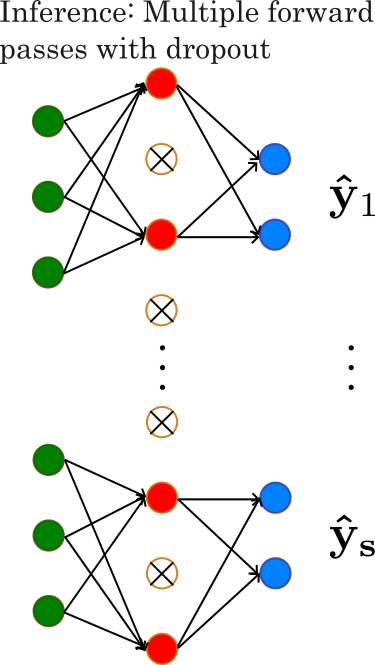
\includegraphics[width=0.33\textwidth]{figures/mcdropout.png}}%
      \begin{subfigure}{0.24\textwidth}
        \raisebox{\dimexpr.5\ht\largestimage-.5\height}{%
        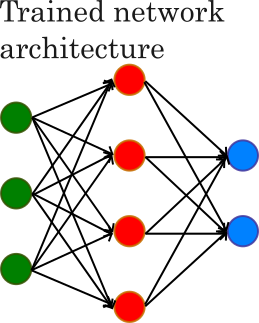
\includegraphics[width=\linewidth]{figures/mcdrop.png}}
        \caption{Original network}
        \label{fig:mcdrop1}
      \end{subfigure}
      \hfill
      \begin{subfigure}{0.33\textwidth}
        \usebox{\largestimage}
        \caption{MC Dropout}
        \label{fig:mcdrop2}
      \end{subfigure}
      \hfill
      \begin{subfigure}{0.33\textwidth}
        \raisebox{\dimexpr\ht\largestimage-\height}{%
        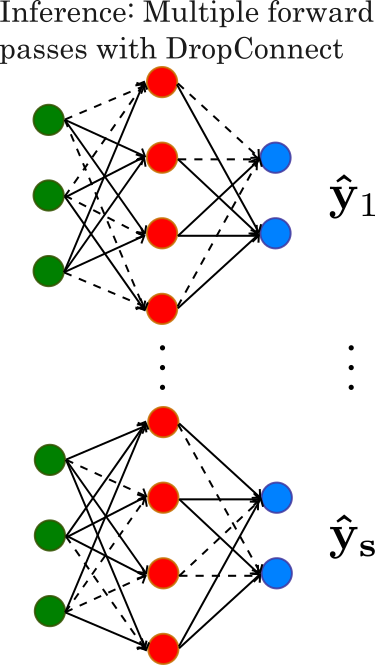
\includegraphics[width=\linewidth]{figures/mcdropconnect.png}}
        \caption{MC DropConnect}
        \label{fig:mcdrop3}
      \end{subfigure}
      \caption{Model uncertainty quantification using Monte Carlo dropout or DropConnect.}
      \label{fig:mcdrop}
    \end{figure}
    Dropout was introduced by~\cite{DropoutOG} as a stochastic regularization technique in NNs to prevent overfitting. By the properties of how dropout (randomly dropping out hidden units of inner layers in NN) is implemented, it also allows one to efficiently combine exponentially many different NNs without extra cost~\cite{DropoutOG}. Mathematically, for an input $x \in \mathbb{R}^d$ and a weight matrix $W\in \mathbb{R}^{d \times d'}$, a masking vector $m \in \mathbb{R}^{d'}$ is sampled whose each element is sampled independently from a Bernoulli distribution with some chosen probability $p$, then the hidden layer can be computed with activation function $a$ as $h = m \star a(Wx)$, where $\star$ refers to element-wise multiplication in this work.
    \newline

    DropConnect, the generalization of Dropout, was introduced by~\cite{DropConnectOG}. Similar to dropout, DropConnect also introduces randomness in the NN, but by randomly dropping a weight (a connection between two hidden units) instead of the hidden units. Mathematically, for an input $x \in \mathbb{R}^d$ and a weight matrix $W\in \mathbb{R}^{d \times d'}$, a masking matrix $M \in \mathbb{R}^{d \times d'}$ is sampled whose each element is sampled independently from a Bernoulli distribution with some chosen probability $p$, then the hidden layer can be computed with activation function $a$ as $h = a((M \star W) x)$.
    \newline

    ~\cite{DropoutUQ} showed that any NN of arbitrary depth with dropout or DropConnect incorporated into it approximates a familiar probabilistic model, namely deep Gaussian Process introduced in~\cite{DeepGP}.~\cite{DropConnectUQ} also showed a computationally tractable approximation of
    a Bayesian Neural Network (BNN) by using DropConnect. Such a probabilistic view allows one to estimate uncertainty using NNs with dropout or DropConnect~\cite{DropoutUQ, DropConnectUQ}. The mean and standard deviation associated with the prediction were empirically estimated for a test sample. The mathematical expression for this, when DropConnect is used, is provided, since it is the generalization of dropout. For a NN with the set of model weights $\theta = \{\theta_1, \ldots, \theta_M\}$, an $M$-dimensional vector of variables each following a Bernoulli distribution $S$ times $\{z^s_1, \ldots, z^s_M\}_{s=1}^S = \{z^s\}_{s=1}^S$ is sampled, corresponding to the model weights after dropping connections as $\{\theta^s_1, \ldots, \theta^s_M\}_{s=1}^S = \{\theta^s\}_{s=1}^S$. Then the mean can be estimated using the approximation given by Eq.~\ref{approxpreddist} as:
    \begin{equation}\label{MCDropMean}
        \mathbb{E}_{q(\mathbf{y^*|x^*})}(\mathbf{y^*}) \approx \frac{1}{S} \sum_{s=1}^S \mathbf{\hat{y}^*(x^*,\theta^s)}
    \end{equation}
    where $\mathbf{\hat{y}^*(x^*,\theta^s)}$ denotes the prediction of the NN with weights $\theta^s$ after DropConnect corresponding to the vector $z^s=\{z^s_1, \ldots, z^s_M\}$. This is equivalent to performing the NN forward pass $S$ times with different DropConnect sampling and averaging the predictions. This Monte Carlo estimate was termed MC DropConnect~\cite{DropConnectUQ} (MC Dropout~\cite{DropoutUQ} when dropout is used). Given that the data uncertainty $Cov_{p(\mathbf{y^*|x^*, \theta})}(y^*) = \sigma^2I$ is known, the predictive covariance can also be estimated as:
    \begin{equation}\label{MCDropVar}
        \mathbf{Var}_{q(\mathbf{y^*|x^*})}(\mathbf{y^*}) \approx \sigma^2I + \frac{1}{S} \sum_{s=1}^S \mathbf{\hat{y}^*(x^*,\theta^s)}^T \mathbf{\hat{y}^*(x^*,\theta^s)} - \mathbb{E}_{q(\mathbf{y^*|x^*})}(\mathbf{y^*})^T \mathbb{E}_{q(\mathbf{y^*|x^*})}(\mathbf{y^*})
    \end{equation}
    which comes from calculating the sample variance of the predictions from $S$ forward passes through the NN, with additional prediction uncertainty coming from the data (which can be ignored if assumed deterministic). Observe that for dropout, an $N$-dimensional vector of variables is sampled with each element sampled from a Bernoulli distribution where $N$ is the number of hidden nodes in the NN. The masked weights after dropout can be similarly computed based on the dropped hidden units instead of the dropped connections, and the same formulations given in Eq.~\ref{MCDropMean} and Eq.~\ref{MCDropVar} can be used to compute the empirical posterior mean and variance, respectively.
    \newline

    MC dropout or MC DropConnect has been a popular method in quantifying model uncertainty due to its simplicity and efficiency. There is no need to use a separate NN for approximation. With minimal modification to the existing network architecture, the uncertainty estimates can be computed by performing multiple forward passes during inference. As a result, there is no need to compromise accuracy by using approximate models. The authors of~\cite{BayesCNN} showed that simple dropout-based approximation fails for certain NN architectures such as Convolutional Neural Networks (CNNs), but the Bayesian interpretation of dropout (MC dropout approximation) helps alleviate this issue. But since all the NNs generated through dropout essentially come from the same parent NN, such methods are often limited in terms of capturing the diversity and approximating the original posterior, leading to underestimated variance and therefore poor uncertainty estimates as shown in~\cite{DropoutIssues1, DropoutIssues2}. For better estimates, many forward passes are required to be performed, which nullifies the cost-effectiveness of such methods~\cite{BayesCNN}. One also needs to be careful with the percentage of sparsity incorporated in the network via dropping out (e.g., high probability of dropping, or using dropout in every layer) as it might impose too strong regularization, resulting in slow learning and decreased accuracy~\cite{BayesSegNetUnc}. Still, due to the scalability in our use case, where we use deep learning models with many parameters, MC dropout or DropConnect are preferred instead of analytic approximation methods.
    


    \subsection{Deep Ensemble}\label{Deepsemble}
    An ensemble model combines the predictions of multiple individual models in some structured way to obtain the final prediction for an input. With the usage of accurate and diverse models, it can be assumed that the ensemble model achieves higher predictive accuracy than the individual models~\cite{EnsembleNN}. This holds for deep learning models too, as shown in~\cite{EnsembleNN, EnsembleNN2, EnsembleNN3}. Ensemble methods can not only improve predictive performance but also provide better-calibrated and more robust uncertainty estimates with capabilities to detect out-of-distribution (OOD) samples, as shown for Deep Ensembles introduced by~\cite{DeepEnsembleUQ}. Deep ensemble combines multiple deep NNs along with adversarial training~\cite{Adversarial} to smooth predictive distribution. Through the combination of multiple NNs, the deep ensemble also provides an empirical distribution over the predictions. So for an ensemble of $M$ NNs with weights or parameter sets $\theta_1, \ldots, \theta_M$ respectively, the predictive probability of output $\mathbf{y^*}$ given an input $\mathbf{x^*}$ can be computed as:
    \begin{equation}\label{EnsemblePred}
        p(\mathbf{y^*|x^*}) = \frac{1}{M} \sum_{m=1}^M p_{\theta_m}(\mathbf{y^*|x^*, \theta_m})
    \end{equation}
    for a uniformly weighted combination of the individual NN predictive probabilities parametrized by $\theta_m$ for $m \in \{1, \ldots, M\}$. In this frequentist approach, the prediction can be empirically estimated by averaging the predictions of the individual NNs, and the uncertainty can be computed by calculating the variance of these output predictions.
    \newline

    Several strategies for creating ensembles have been developed over the years. A review of general-purpose methods of constructing ensemble models can be found in~\cite{EnsembleReview}. For NNs, this can be differentiated based on the sources of uncertainty one wants to capture. An ensemble of different neural networks (NNs) can be constructed by using different parameter initializations, varying hyperparameters (e.g., learning rate, optimization strategy, regularization parameter)~\cite{HyperparEnsUnc}, or adjusting the number of layers, hidden nodes, or activation function. One can also keep the same NN architecture across different models, but randomize the data to learn different parameters by random shuffling of datasets or bootstrapping~\cite{DeepEnsembleUQ, NeuBoots}.
    \newline

    Like the dropout-based methods, deep ensemble methods are also easy to implement for estimating uncertainty. During training and inference, the process can be parallelized by training or inferring from each model separately at the same time. However, these methods still have a high computational and memory costs, which increase linearly with the number of models used in the ensemble in both training and inference, since one has to train or infer from and store multiple independent models in parallel. One also needs enough model diversity to ensure better uncertainty estimation from ensemble models. Several approaches have been developed~\cite{BatchEnsemble, Masksembles, PackedEnsemble} to address the bottleneck of memory and computational cost of standard ensemble methods. BatchEnsemble~\cite{BatchEnsemble} used efficient parametrization by using a shared weight matrix for all models and a rank-one matrix varying across different models for each connected layer, and therefore creates a member of the ensemble at each layer, which can be trained simultaneously. Masksembles~\cite{Masksembles} borrowed the idea of MC dropout, but instead of randomly dropping weights or nodes of the NN, Masksembles used a finite number of carefully chosen binary masks to be applied during training and inference. Packed-Ensembles~\cite{PackedEnsemble} used grouped convolutions proposed in AlexNet~\cite{AlexNet} to independently train subnetworks with fewer parameters within one base model.



\section{Implicit Generative Models}\label{ImplicitGen}
\begin{figure}[htb]
  \begin{center}
  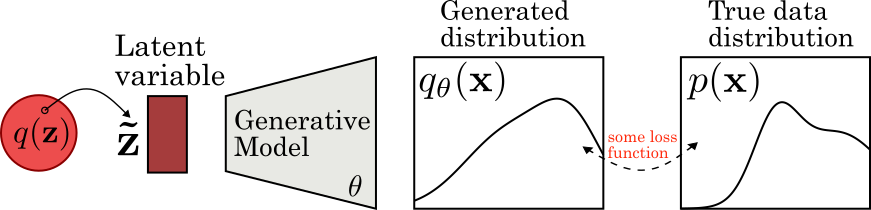
\includegraphics[width=\linewidth]{figures/implicitgen.png}
  \end{center}
  \caption{Learning implicit generative models.}\label{fig:implicit_gen}
\end{figure}
An implicit generative model is a stochastic process that can be used to directly simulate data from a probability distribution, and therefore it implicitly defines a probability distribution. As implicit generative models do not provide an explicit parametric specification of the
distribution of an observed random variable $\mathbf{x}\in \mathbb{R}^d$, the likelihood is often intractable. These models can also be thought of as latent variable models since they use a latent variable $\mathbf{\tilde{z}} \in \mathbb{R}^m$ and apply a deterministic function $\mathcal{G}_\theta: \mathbb{R}^m\rightarrow \mathbb{R}^d$ parametrized by $\theta$ on the latent variable $\mathbf{\tilde{z}}$ mapping it to a sample in the distribution. This can be formulated as:
\begin{equation}\label{IGM}
    \mathbf{\tilde{z}} \sim q(\mathbf{z}), \quad \mathbf{x} =  \mathcal{G}_\theta(\mathbf{\tilde{z}})
\end{equation}
where the latent variable is generated from a fixed, simple distribution such as a standard Gaussian ($\mathbf{\tilde{z}} \sim \mathcal{N}\left(0, I_m\right)$). We can effectively approximate the original data distribution $p(\mathbf{x})$ by computing the likelihood specified by Eq.~\ref{IGM}:
\begin{equation}\label{IGMLikelihood}
    p(\mathbf{x}) \approx q_\theta(\mathbf{x}) = \frac{\partial}{\partial x_1} \cdots \frac{\partial}{\partial x_d} \int_{\mathcal{G}_\theta(\mathbf{z}) \leq \mathbf{x}} q(\mathbf{z}) d\mathbf{z}
\end{equation}
for $\mathbf{x}=\{x_1, \ldots, x_d\}$. 
\\
If $\mathcal{G}$ is invertible, or has easily characterised roots with the data space having the same dimension as the latent space, the rules of transformation of probability density can be applied to compute the generated distribution~\cite{LearnIGM}. But such functions limit the capabilities of modelling more complex distributions. Therefore, more general functions are preferred, such as a differentiable function specified by a deep NN. In such cases, Eq.~\ref{IGMLikelihood} is often intractable. Therefore, methods that approximate the likelihood in Eq~\ref{IGMLikelihood} or completely avoid using the likelihood must be implemented. An extensive discussion about such methods is done in~\cite{LearnIGM}.


    

\section{Gaussian Process}\label{GP}
A Gaussian process (GP) is a generalization of the Gaussian distribution extended to an infinite number of dimensions. A probability distribution describes the probability of different values (scalar or vector) a random variable (univariate or multivariate) can take. On the other hand, a stochastic process determines the properties a random function follows. According to the above definitions, a Gaussian process can be considered as a stochastic process over infinite-dimensional functions or an infinite collection of random variables, any finite number of which follow a joint Gaussian distribution~\cite{GPML}. So, given a finite set of points, a Gaussian process can provide us probability distribution over possible functions that fit those points. Evidently, GP is a non-parametric model. 
\newline

Now, let $\mathcal{F}=\{f(\mathbf{x})\}_{\mathbf{x} \in D}$ be a collection of random variables for some continuous value $\mathbf{x} \in D \subset \mathbb{R}^d$. Therefore by definition, $\mathcal{F}$ is a Gaussian process if for any two values $\mathbf{x}, \mathbf{x}^{\prime} \in D \subset \mathbb{R}^d$,

\begin{equation}\label{GPDef}
    f(\mathbf{x}), f\left(\mathbf{x}^{\prime}\right) \sim \mathcal{N}\left(\left[\begin{array}{c}
    m(\mathbf{x})  \tag{1}\\
    m\left(\mathbf{x}^{\prime}\right)
    \end{array}\right],\left[\begin{array}{cc}
    k(\mathbf{x}, \mathbf{x}) & k\left(\mathbf{x}, \mathbf{x}^{\prime}\right) \\
    k\left(\mathbf{x}^{\prime}, \mathbf{x}\right) & k\left(\mathbf{x}^{\prime}, \mathbf{x}^{\prime}\right)
    \end{array}\right]\right)
\end{equation}
for some mean function $m(\mathbf{x})$ and covariance function $k\left(\mathbf{x}, \mathbf{x}^{\prime}\right)$ where $m: D \rightarrow \mathbb{R}, k: D \times D \rightarrow \mathbb{R}$ uniquely specify the Gaussian process $\mathcal{F}$. The mean and the covariance functions of the actual Gaussian process $f(\mathbf{x})$ can be defined as:
\begin{align}\label{GPFunc}
    m(\mathbf{x}) & =\mathbb{E}[f(\mathbf{x})]  \\
    k\left(\mathbf{x}, \mathbf{x}^{\prime}\right) & =\mathbb{E}\left[(f(\mathbf{x})-m(\mathbf{x}))\left(f\left(\mathbf{x}^{\prime}\right)-m\left(\mathbf{x}^{\prime}\right)\right)\right]
\end{align}
The Gaussian process is denoted as:
\begin{equation}\label{GPForm}
f(\mathbf{x}) \sim \mathcal{G} \mathcal{P}\left(m(\mathbf{x}), k\left(\mathbf{x}, \mathbf{x}^{\prime}\right)\right)
\end{equation}
Given a dataset $\mathbf{X=\{x_n\}_{n=1}^N, Y=\{y_n\}_{n=1}^N}$, where $\forall n \in \{1, \ldots, N\}$, $\mathbf{y_n}$ is an observed instance of the GP defined by the function $f$, and a set of new points $\mathbf{X^*=\{x^*_n\}_{n=1}^{N^*}}$ the joint distribution of the test points and observed points $\left[f(\mathbf{X^*, X})\right]^T$=$\left[f\left(\mathbf{x^*}_{1}\right), \ldots, f\left(\mathbf{x^*_{N^*}}\right), f\left(\mathbf{x}_{1}\right), \ldots, f\left(\mathbf{x_{N}}\right)\right]^T$ according to the GP prior can be written as:
{\small\begingroup
\renewcommand{\arraystretch}{1.25}
\setlength\arraycolsep{0.5pt}
\begin{equation}\label{GPJointBig}
    \mathcal{N}\left(\left[\begin{array}{c}
        m\left(\mathbf{x^*}_{1}\right)\\
        \vdots \\
        m\left(\mathbf{x^*_{N^*}}\right)\\
        m\left(\mathbf{x}_{1}\right)\\
        \vdots \\
        m\left(\mathbf{x_{N}}\right)
        \end{array}\right],
        \left[
        \begin{array}{cccccc}
        k\left(\mathbf{x^*}_{1}, \mathbf{x^*}_{1}\right) & \ldots & k\left(\mathbf{x^*}_{1}, \mathbf{x^*}_{N^*}\right) & k\left(\mathbf{x^*}_{1}, \mathbf{x}_{1}\right) & \ldots & k\left(\mathbf{x^*}_{1}, \mathbf{x}_{N}\right) \\
         \vdots & \ddots & \vdots & \vdots & \ddots & \vdots \\
        k\left(\mathbf{x^*}_{N^*}, \mathbf{x^*}_{1}\right) & \ldots & k\left(\mathbf{x^*}_{N^*}, \mathbf{x^*}_{N^*}\right) & k\left(\mathbf{x^*}_{N^*}, \mathbf{x}_{1}\right) & \ldots & k\left(\mathbf{x^*}_{N^*}, \mathbf{x}_{N}\right) \\
        k\left(\mathbf{x}_{1}, \mathbf{x^*}_{1}\right) & \ldots & k\left(\mathbf{x}_{1}, \mathbf{x^*}_{N^*}\right) & k\left(\mathbf{x}_{1}, \mathbf{x}_{1}\right) & \ldots & k\left(\mathbf{x}_{1}, \mathbf{x}_{N}\right) \\
        \vdots & \ddots & \vdots & \vdots & \ddots & \vdots \\
        k\left(\mathbf{x}_{N}, \mathbf{x^*}_{1}\right) & \ldots & k\left(\mathbf{x}_{N}, \mathbf{x^*}_{N^*}\right) & k\left(\mathbf{x}_{N}, \mathbf{x}_{1}\right) & \ldots & k\left(\mathbf{x}_{N}, \mathbf{x}_{N}\right)
        \end{array}
        \right]\right)
\end{equation}
\endgroup
}
which can be rewritten as
\begin{equation}\label{GPJointConcise}
        \left[\begin{array}{l}
        f\left(\mathbf{X^*}\right)\\
        f\left(\mathbf{X}\right)
    \end{array}\right] \sim \mathcal{N}\left(\left[\begin{array}{c}
        m\left(\mathbf{X^*}\right)\\
        m\left(\mathbf{X}\right)
        \end{array}\right],
        \left[\begin{array}{cc}
        k\left(\mathbf{X^*}, \mathbf{X^*}\right) & k\left(\mathbf{X^*}, \mathbf{X}\right) \\
        k\left(\mathbf{X}, \mathbf{X^*}\right) & k\left(\mathbf{X}, \mathbf{X}\right) \\
        \end{array}\right]\right)
\end{equation}
From this probabilistic formulation, the posterior distribution over functions for new pointd can be easily computed by conditioning the joint prior distribution on the observations:
\begin{equation}\label{GPPosterior}
    \begin{aligned}
        f\left(\mathbf{X^*} \mid \mathbf{X, Y}\right) \sim \mathcal{N}(m\left(\mathbf{X^*}\right)+k\left(\mathbf{X^*}, \mathbf{X}\right) k\left(\mathbf{X}, \mathbf{X}\right)^{-1}\left(\mathbf{Y}-m\left(\mathbf{X}\right)\right),\\
        k\left(\mathbf{X^*}, \mathbf{X^*}\right)-k\left(\mathbf{X^*}, \mathbf{X}\right) k\left(\mathbf{X}, \mathbf{X}\right)^{-1} k\left(\mathbf{X}, \mathbf{X^*}\right))
    \end{aligned}
\end{equation}
Usually, a zero mean ($m(\mathbf{x})=0$) is assumed for the GP prior. If the mean is not zero, the data can always be centred, or the Gaussian process $f-m$ can be considered. In case of a zero mean prior, the posterior in Eq.~\ref{GPPosterior} becomes:
\begin{equation}\label{GPPosterior0}
    \begin{aligned}
        f\left(\mathbf{X^*}\right) \mid \mathbf{X, Y} \sim \mathcal{N}(k\left(\mathbf{X^*}, \mathbf{X}\right) k\left(\mathbf{X}, \mathbf{X}\right)^{-1}\mathbf{Y}, \\
        k\left(\mathbf{X^*}, \mathbf{X^*}\right)-k\left(\mathbf{X^*}, \mathbf{X}\right) k\left(\mathbf{X}, \mathbf{X}\right)^{-1} k\left(\mathbf{X}, \mathbf{X^*}\right))
    \end{aligned}
\end{equation}
\newline

However, in real-life settings, one does not have access to the ground-truth function values. Only some noisy values are observed which can be modelled as $\mathbf{y} = f(\mathbf{x}) + \varepsilon$ for some observed input $\mathbf{x}$ where the noise $\varepsilon$ is assumed to follow a Gaussian distribution, $\varepsilon \sim \mathcal{N}(0, \sigma^2_N I)$ for the $N$ observed data points. It is known that the sum of two Gaussian distributions is also Gaussian for two independent Gaussian random variables with the mean and the covariance equal to the sum of the means and covariances of the two Gaussians. Therefore, for the independent identically distributed Gaussian noise, the prior covariance becomes $k\left(\mathbf{X^*}, \mathbf{X^*}\right) + \sigma^2_N I$, and then the joint distribution and the posterior can be rewritten by replacing $k\left(\mathbf{X^*}, \mathbf{X^*}\right)$  with $k\left(\mathbf{X^*}, \mathbf{X^*}\right) + \sigma^2_N I$.
\newline

The covariance function is a critical component of a Gaussian process since it encodes the prior assumptions about the function to be learnt regarding similarity between the data points~\cite{GPML}. Intuitively, similar inputs are expected to have similar outputs. The covariance function indicates how closely a certain input is related to other observed points, and only the close points will have significant contributions to the output prediction. There are many possible choices for the covariance function depending on the application and our prior knowledge about the function. A comprehensive list of potential covariance functions can be found in~\cite{GPML}.


\section{Contrastive Learning}\label{Contrast}
Contrastive learning is a method of learning an embedding space from data that maintains the pairwise similarity between data points. The idea is to find a function that maps inputs into outputs in a target space, such that similar pairs remain similar according to some similarity metric and dissimilar pairs are separated. The target embedding space approximates the semantic distance inherent in the input space. One can observe that contrastive learning only requires semantic relationships of similarity and does not need any distance measure in the input space~\cite{PairMarginCL}. Such a mapping can be learnt by minimizing an appropriate discriminative loss function, called the contrastive loss function. One of the earliest works to introduce such an objective~\cite{ContLoss} applied contrastive learning to a face verification task.~\cite{PairMarginCL} used the same idea for dimensionality reduction, which is useful for dealing with high-dimensional data similar to this work. Due to numerical precision issues encountered in computing the Gaussian process posterior or even marginal likelihood, contrastive learning can provide an alternative approach to learn a feature mapping for points without requiring likelihood computation, as a means of prior separation of dissimilar points before modeling a GP. Moreover, although contrastive learning has been more impactful in self-supervised learning, recent works have also seen a rise in applications in supervised learning~\cite{SelfSupervisedCont, SupervisedCont}. 
\newline

Earlier works mostly focused on loss involving pairs (positive and negative) of samples, but later works have introduced various new contrastive loss functions useful for different applications. In this work, the contrastive losses used will be the triplet loss introduced in~\cite{TripletLoss}, sigmoid loss used in language-image pair pre-training~\cite{SigLIP}, and a discriminative loss based on spacetime distance used in~\cite{SpaceMesh}.
\newline

Triplet loss considers triplets of data points where an anchor is selected along with a positive and a negative sample for which the function $\mathbf{f}$ maps the positive instance close to the anchor and the negative one farther away according to some distance metric. Euclidean distance is usually selected as the metric in the target space. So for any anchor $\mathbf{x^a_i}$, positive sample $\mathbf{x^p_i}$ and negative sample $\mathbf{x^n_i}$ in a set of triplets $\mathcal{T} = \mathbf{\left(x_{i}^{a}, x_{i}^{p}, x_{i}^{n}\right)_{i=1}^N}$, it is desired that:
\begin{equation}\label{tripletcondition}
    \left\|\mathbf{f(x_{i}^{a})-f(x_{i}^{p})}\right\|_{2}^{2}+\epsilon<\left\|\mathbf{f(x_{i}^{a})-f(x_{i}^{p})}\right\|_{2}^{2}, \forall\left(\mathbf{x_{i}^{a}, x_{i}^{p}, x_{i}^{n}}\right) \in \mathcal{T} 
\end{equation}
where $\epsilon$ is the margin enforced between positive and negative pairs. Then the triplet loss can be defined as:
\begin{equation}\label{tripletloss}
    \mathcal{L}(\mathbf{f}, \mathcal{T}) = \sum_{\mathbf{i=1}}^\mathbf{N} \max \left(\left\|\mathbf{f(x_{i}^{a})-f(x_{i}^{p})}\right\|_{2}^{2} - \left\|\mathbf{f(x_{i}^{a})-f(x_{i}^{n})}\right\|_{2}^{2} +\epsilon, 0\right) .
\end{equation}
\newline

On the other hand, sigmoid loss in language-image pair pre-training and spacetime distance-based contrastive loss cannot be directly used in this work. Details of the modified formulations to these losses are provided in Chapter~\ref{ch:methods}.